\subsection{Exchanging signatures}
Two peers in a network will create their blocks together without having to rely on a third party.
Between the peers one is uploading to the other.
The uploader is traditionally called the seeder in BitTorrent and the receiver of this data the downloader~\cite{Cohen-bittorrent}.
The seeder will initiate the block creation.\,
co the seeder can decide how altruistic it wants to be towards the downloader regarding its collaboration.
We will explain how the block creation protocol works.
A sequence diagram can be seen in Figure \ref{fig:exchange-new-sequence}.

\begin{figure}[tpb]
\centering
\subfigure[Sequence diagram for block creation.]{
\centerline{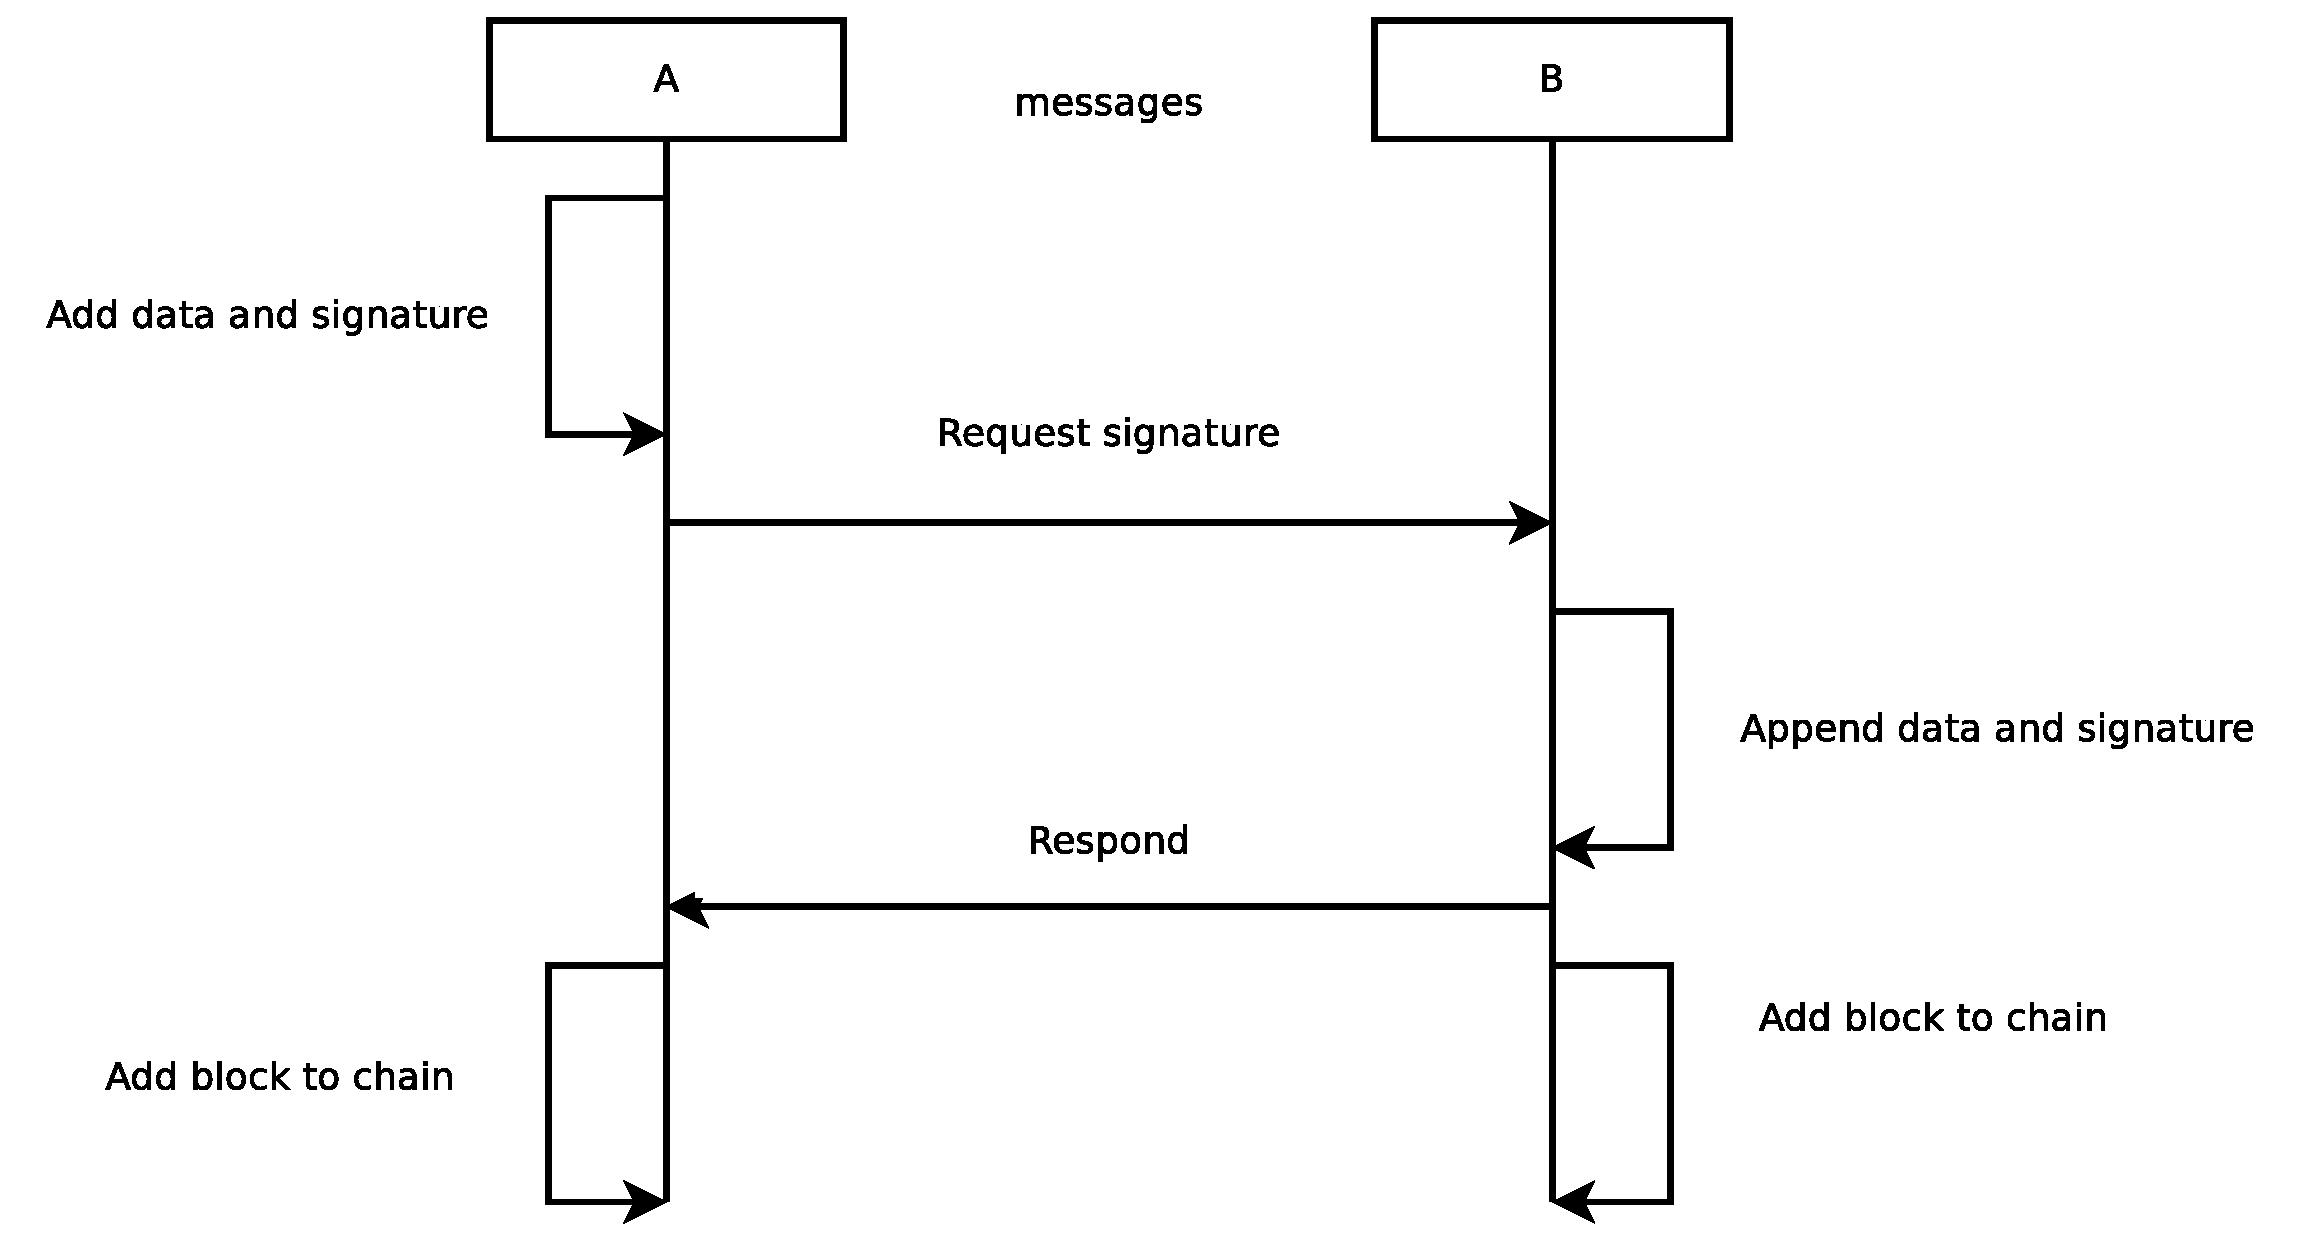
\includegraphics[scale=0.3]{design/figs/exchange_new.eps}}
\label{fig:exchange-new-sequence}
}

\subfigure[Data added by peer A and B for a new block.]{
	\centerline{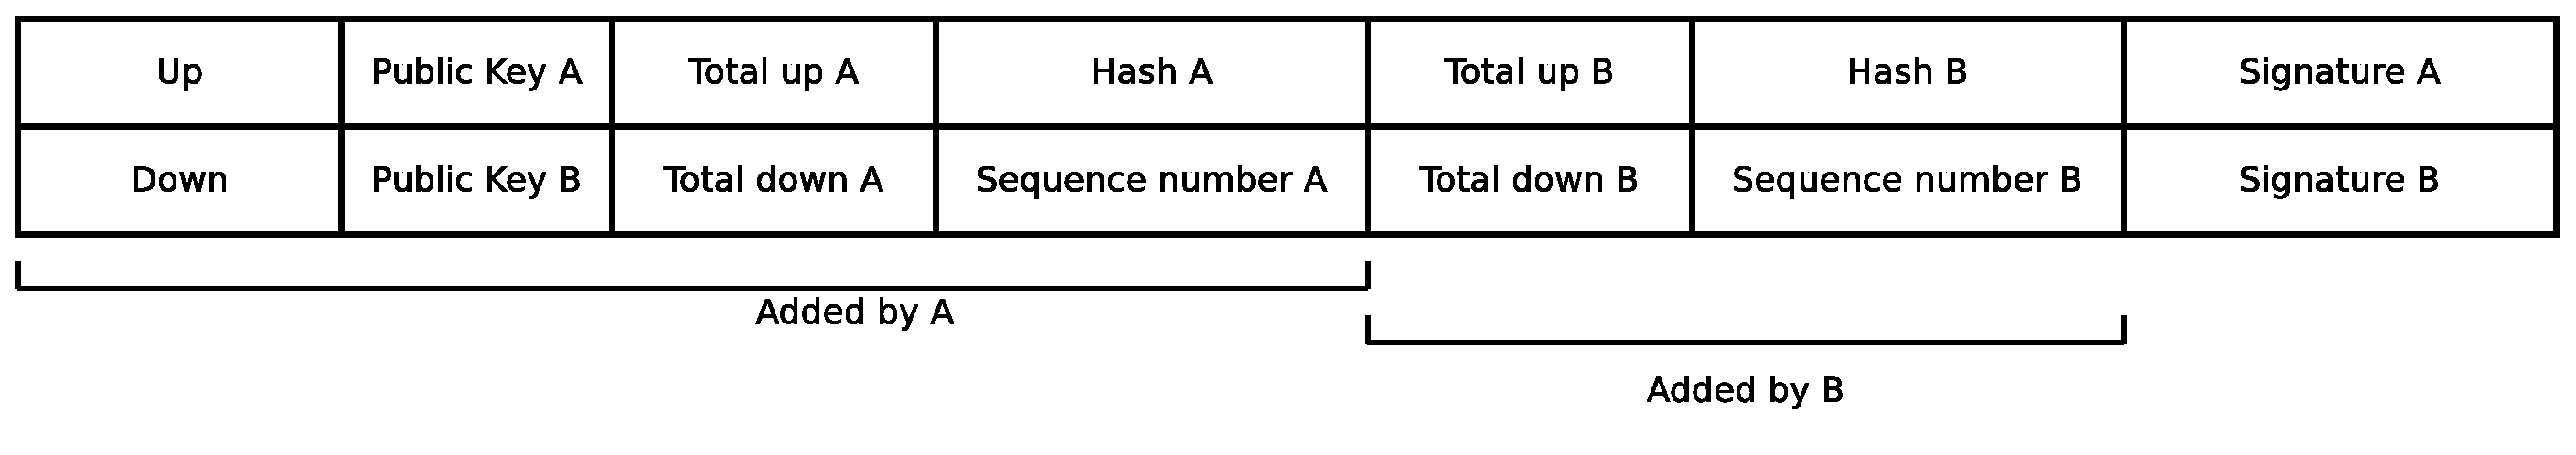
\includegraphics[scale=0.3]{design/figs/packet_creation.eps}}
\label{fig:packet-creation}
}
\caption{Exchanging data with our cleaner design in Dispersy.}
\label{fig:block-creation-new}
\end{figure}

The seeder, A, will create a packet that will be sent to the downloader, B.
A will add to this packet the data uploaded and downloaded data between the peers
that has not yet been added to the MultiChain.
It will add these amounts to its total uploaded and downloaded data
and add these total amounts aswell to the packet.
Finally, it adds the public keys of both peers and its own hash pointer to the packet.
This packet is signed using its private key and sent to the downloader.
The data that A adds can be seen in Figure \ref{fig:packet-creation}.

B will receive this packet and check if the amounts are correct, if the signature is correct,
and if A has not used the previous hash before.
If this is all correct,
then B will add the amounts of uploaded and downloaded data to its own total amounts.
The data contained in the previous packet, the total amounts of B and the hash of the previous block is
inserted into a new packet.
This packet is signed by the private key of B and sent back to A.
The data that B adds can be seen in Figure \ref{fig:packet-creation}.

Both parties now have the data of the block and can add this to their chain and continue forward.
A does this upon receival of the block.
B does this immediatly after sending the return packet to A.
At this point a new block is created.

\subsubsection{Integrating with Dispersy}
\begin{figure}[!h]
\centering
\subfigure[Sequence diagram for block creation.]{
\centerline{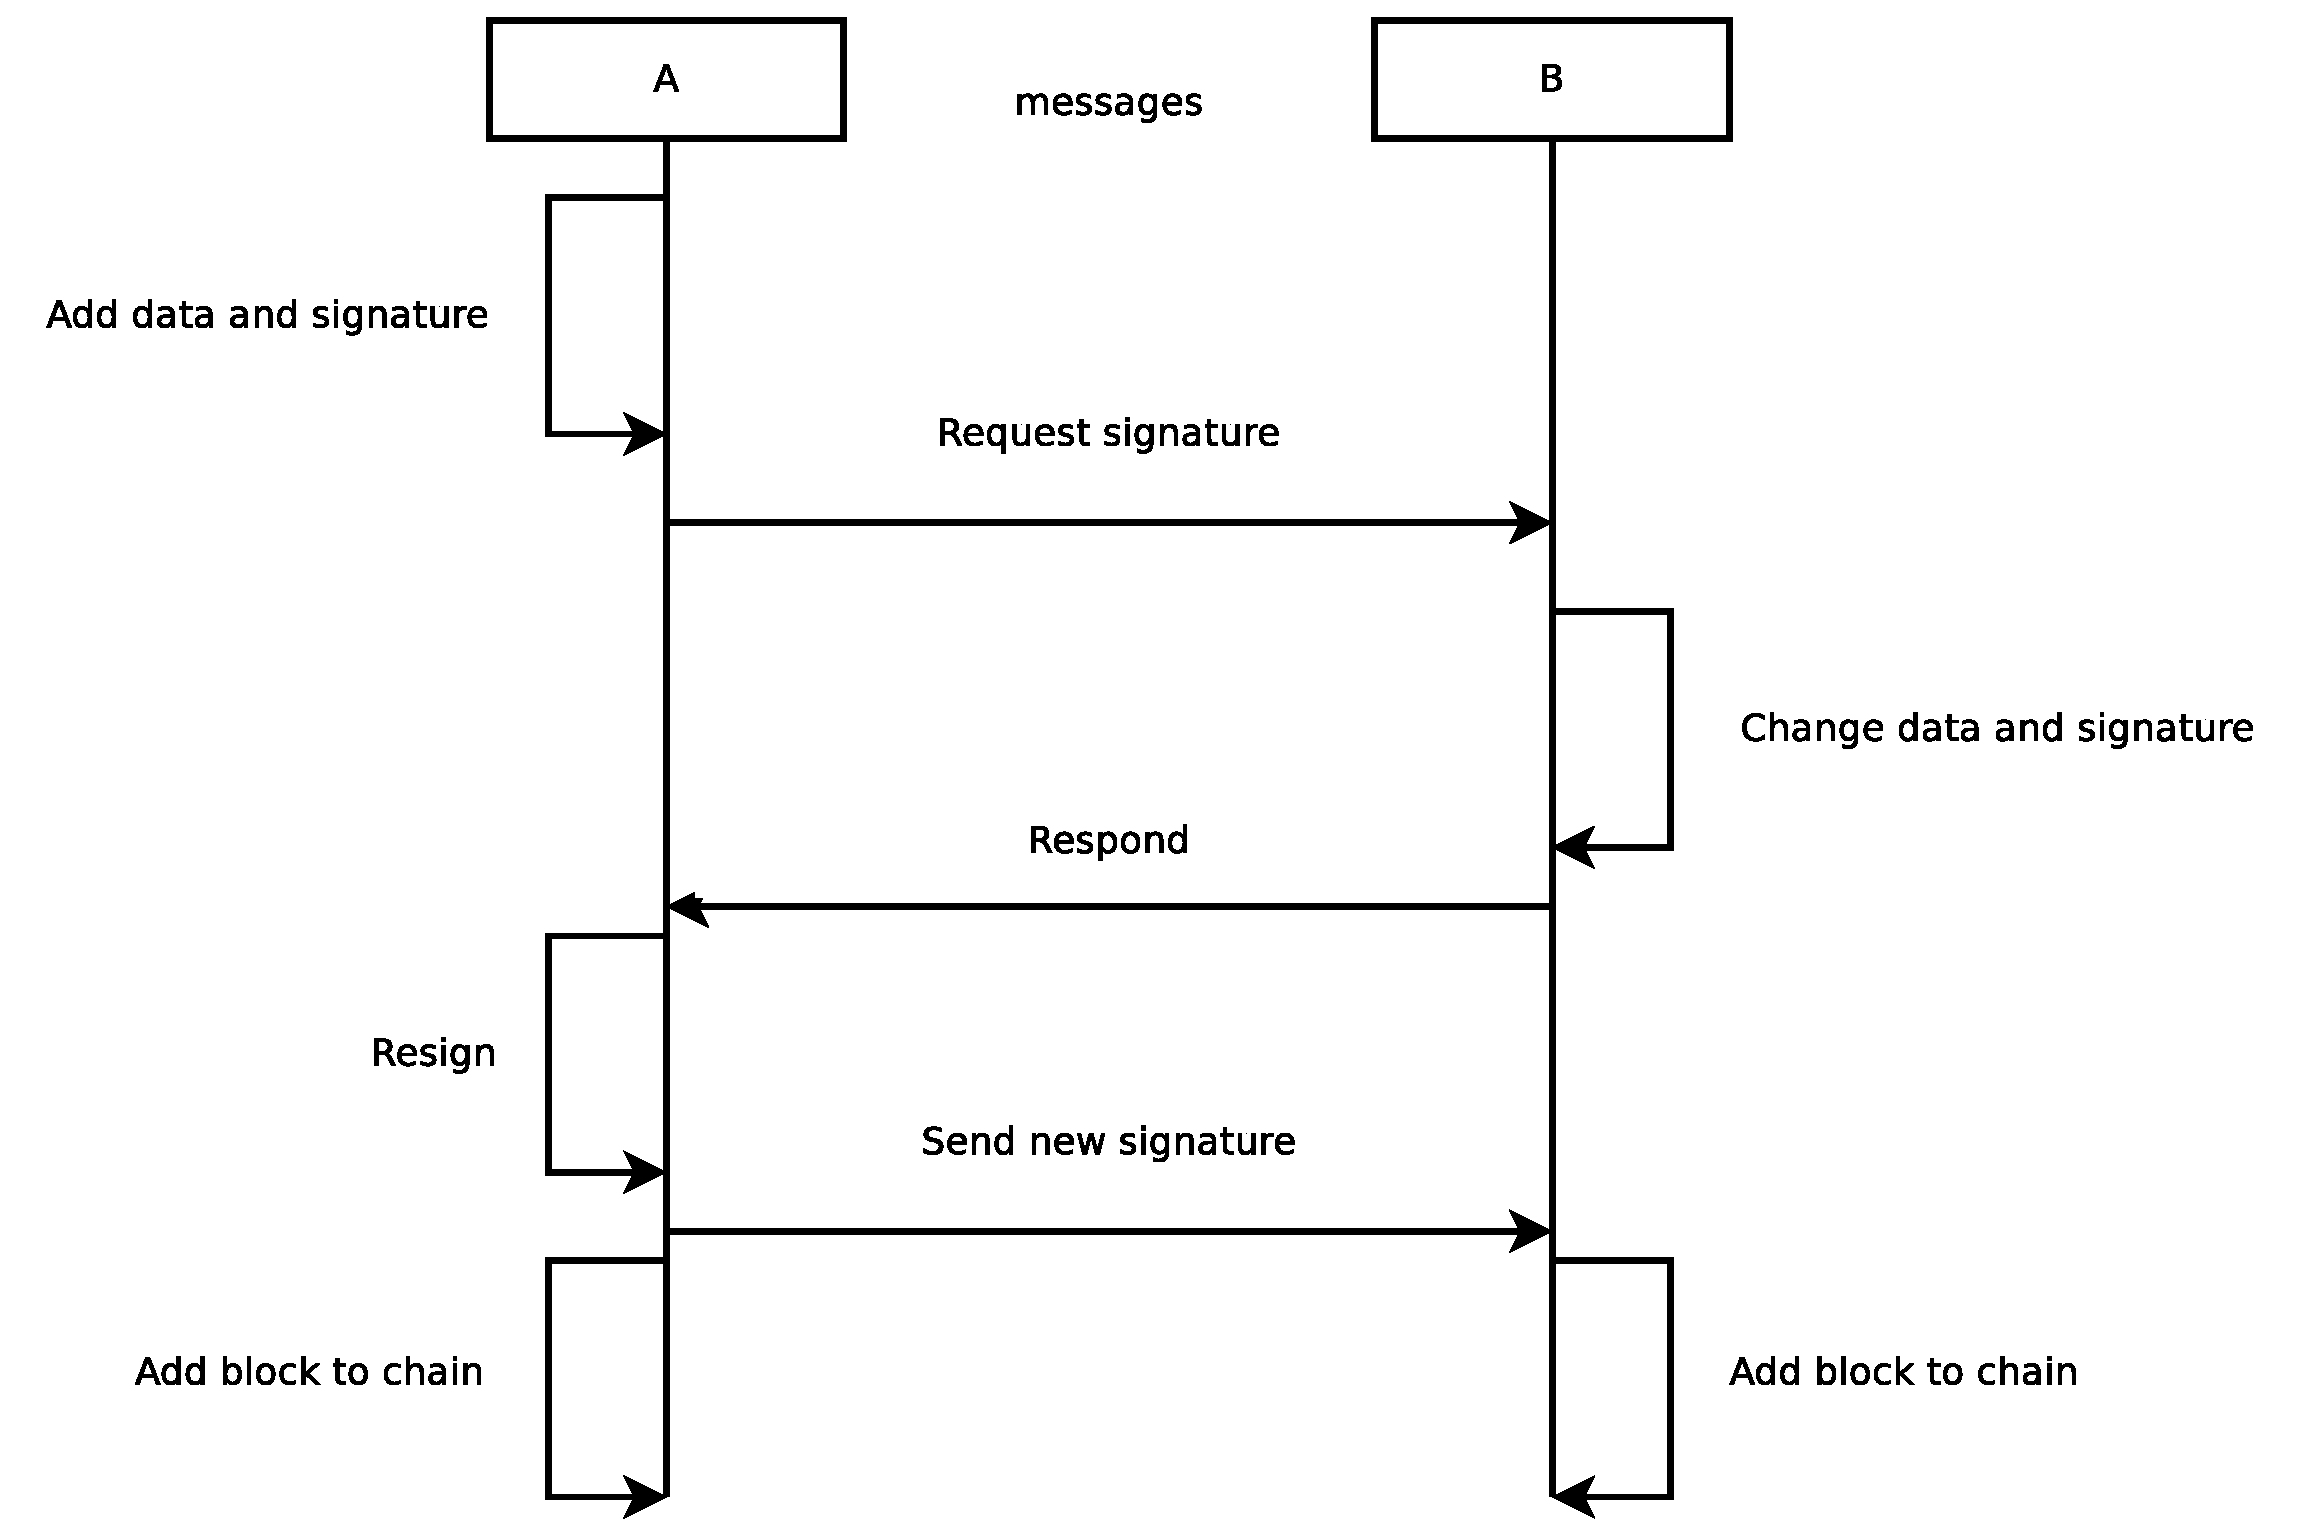
\includegraphics[scale=0.3]{design/figs/exchange_old.eps}}
\label{fig:exchange-old-sequence}
}

\subfigure[Data added by peer A and B for a new block.]{
	\centerline{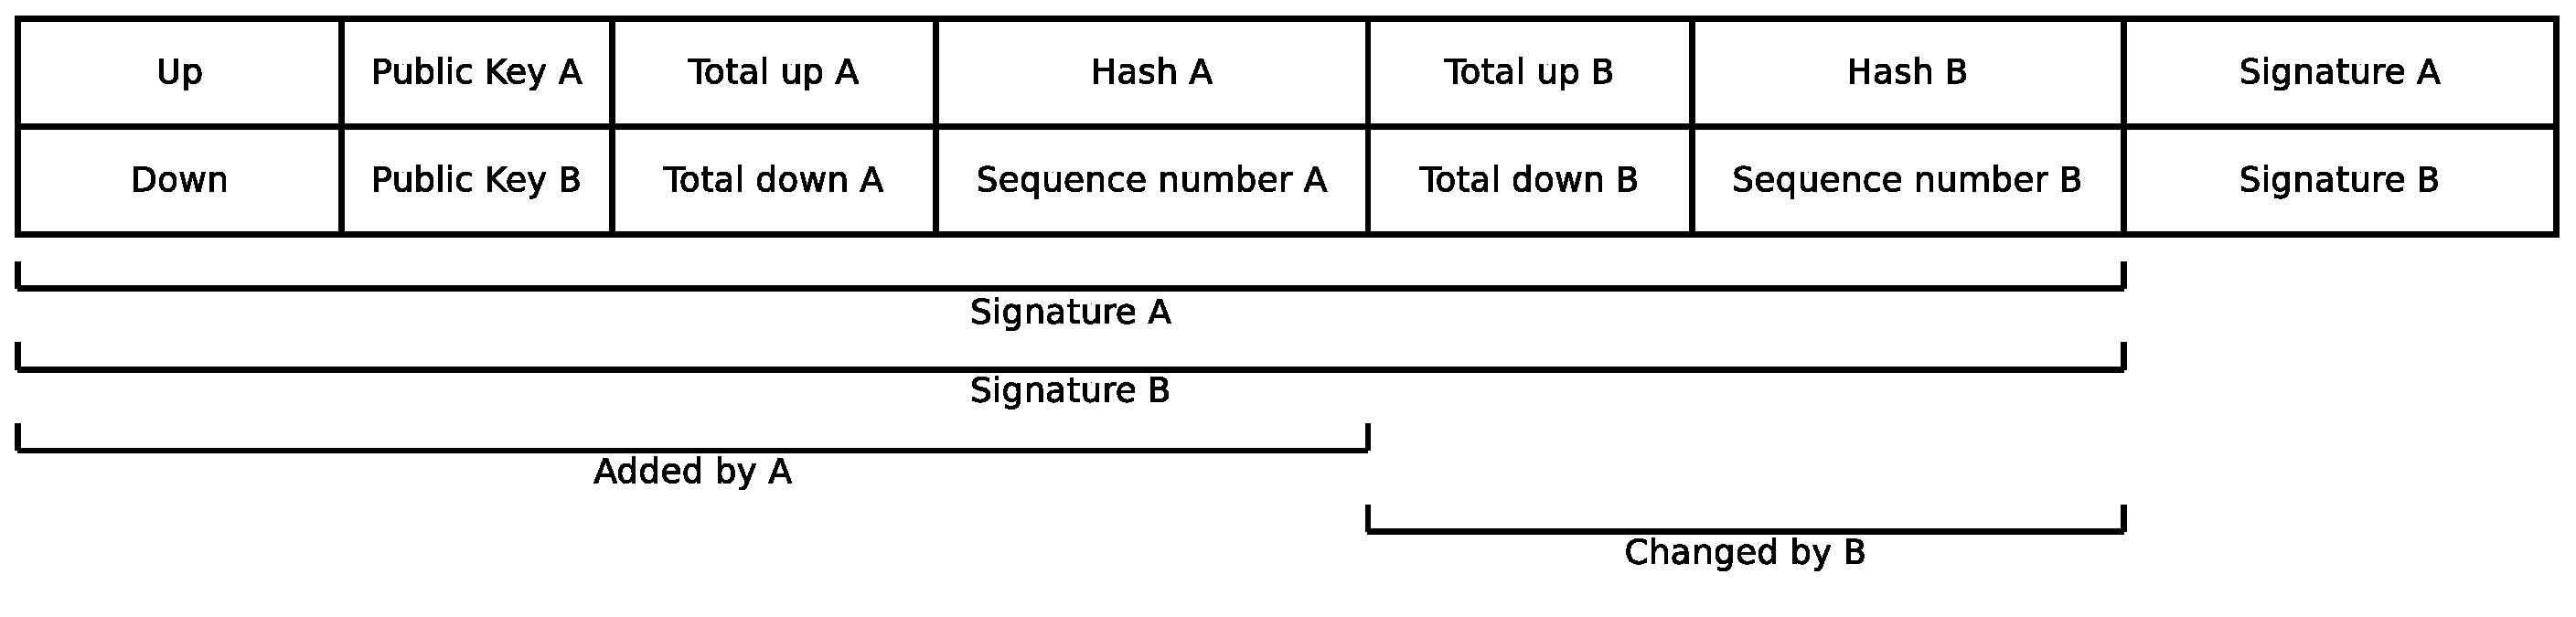
\includegraphics[scale=0.3]{design/figs/signature_old.eps}}
    \label{fig:payload-signature-old}
}
\caption{Exchanging data for block creation using the old design in Dispersy.}
\label{fig:block-creation-old}
\end{figure}
Within Dispersy functionality was already build to create a message, sign the message
and request multiple nodes to also provide their signature on this message.
This existing functionality could be used by MultiChain to exchange signatures
between A and B for the creation of a new block.

A would initiate a message, insert its data into this message, sign the message, and send this message to B.
The functionality would allow B to accept the message and provide its signature or
modify the message and then provide its signature.
Only B knows the hash of its head node, and the total up and total download metrics.
So B will always modify the message and insert its own data in the message.
But this would invalidate the signature of A,
because the signature of A was also placed on the empty part of the message where the data of B is inserted.
The contents of the message and who signs what can be seen in Figure \ref{fig:payload-signature-old}.

After B returns the message,
A would have to resign the message.
But B also needs this valid signature from A before it can add the block to its own chain.
So A would need to send a third message to with the new, valid signature back to B.
A sequence diagram can be seen in Figure \ref{fig:exchange-old-sequence} of how it would work in Dispersy.
Functionality was added to Dispersy that allows to append data in a signature request.
This allows the full signature exchange to be achieved within two messages.